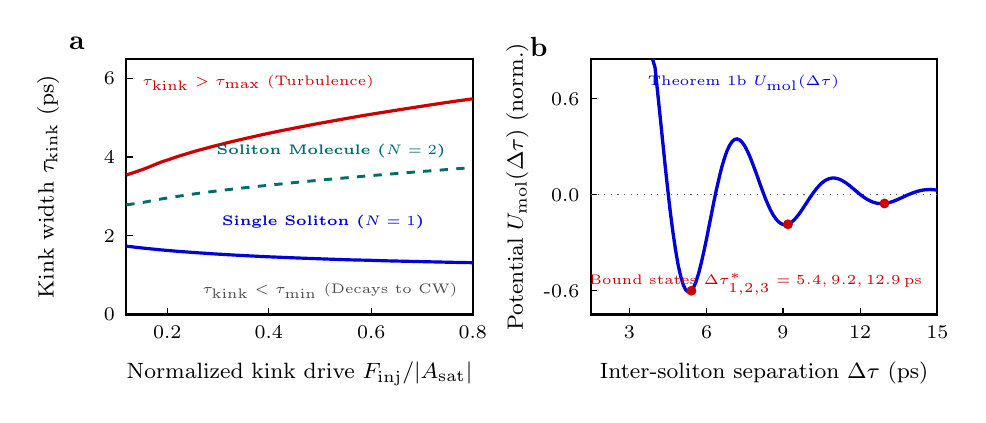
\begin{tikzpicture}[x=1cm,y=1cm,font=\footnotesize]
  % Panel a: Phase-Kink Nucleation Window (tau_kink vs F_inj)
  \node[anchor=north west,font=\bfseries\normalsize] at (0.10,4.35) {a};
  \draw[thick] (0.95,0.70) rectangle (5.35,3.95);
  \foreach \v/\y in {0/0.70, 2/1.70, 4/2.70, 6/3.70} {
    \draw (0.95,\y) -- (1.03,\y);
    \node[left,font=\scriptsize] at (0.93,\y) {\v};
  }
  \foreach \xval/\xpos in {0.2/1.47, 0.4/2.76, 0.6/4.06, 0.8/5.35} {
    \draw (\xpos,0.70) -- (\xpos,0.78);
    \node[below,font=\scriptsize] at (\xpos,0.68) {\xval};
  }
  \node[below,font=\footnotesize] at (3.15,0.22) {Normalized kink drive $F_{\mathrm{inj}}/|A_{\mathrm{sat}}|$};
  \node[rotate=90,above,font=\footnotesize] at (0.22,2.32) {Kink width $\tau_{\mathrm{kink}}$ (ps)};

  \draw[blue!85!black,line width=1.15pt] (0.950,1.568) -- (1.170,1.543) -- (1.390,1.521) -- (1.610,1.502) -- (1.830,1.486) -- (2.050,1.471) -- (2.270,1.458) -- (2.490,1.446) -- (2.710,1.435) -- (2.930,1.426) -- (3.150,1.417) -- (3.370,1.409) -- (3.590,1.401) -- (3.810,1.394) -- (4.030,1.389) -- (4.250,1.382) -- (4.470,1.377) -- (4.690,1.372) -- (4.910,1.367) -- (5.130,1.362) -- (5.350,1.358);
  \draw[red!80!black,line width=1.15pt] (0.950,2.471) -- (1.170,2.546) -- (1.390,2.635) -- (1.610,2.709) -- (1.830,2.776) -- (2.050,2.835) -- (2.270,2.891) -- (2.490,2.942) -- (2.710,2.991) -- (2.930,3.037) -- (3.150,3.080) -- (3.370,3.122) -- (3.590,3.162) -- (3.810,3.201) -- (4.030,3.239) -- (4.250,3.274) -- (4.470,3.309) -- (4.690,3.343) -- (4.910,3.377) -- (5.130,3.409) -- (5.350,3.440);
  \draw[teal!85!black,dashed,line width=1.05pt] (0.950,2.092) -- (1.170,2.125) -- (1.390,2.167) -- (1.610,2.202) -- (1.830,2.234) -- (2.050,2.263) -- (2.270,2.289) -- (2.490,2.314) -- (2.710,2.337) -- (2.930,2.360) -- (3.150,2.382) -- (3.370,2.403) -- (3.590,2.423) -- (3.810,2.442) -- (4.030,2.462) -- (4.250,2.480) -- (4.470,2.498) -- (4.690,2.516) -- (4.910,2.532) -- (5.130,2.550) -- (5.350,2.566);

  \node[font=\tiny\bfseries,blue!85!black] at (3.45,1.88) {Single Soliton ($N=1$)};
  \node[font=\tiny\bfseries,teal!85!black] at (3.55,2.78) {Soliton Molecule ($N=2$)};
  \node[anchor=north west,font=\tiny,red!80!black] at (1.03,3.86) {$\tau_{\mathrm{kink}} > \tau_{\max}$ (Turbulence)};
  \node[anchor=south east,font=\tiny,black!70] at (5.28,0.78) {$\tau_{\mathrm{kink}} < \tau_{\min}$ (Decays to CW)};

  % Panel b: Soliton Molecule Interaction Potential U_mol(Delta tau)
  \node[anchor=north west,font=\bfseries\normalsize] at (5.95,4.35) {b};
  \draw[thick] (6.85,0.70) rectangle (11.25,3.95);
  \foreach \v/\y in {-0.6/1.00, 0.0/2.22, 0.6/3.44} {
    \draw (6.85,\y) -- (6.93,\y);
    \node[left,font=\scriptsize] at (6.83,\y) {\v};
  }
  \foreach \xval/\xpos in {3/7.34, 6/8.32, 9/9.29, 12/10.27, 15/11.25} {
    \draw (\xpos,0.70) -- (\xpos,0.78);
    \node[below,font=\scriptsize] at (\xpos,0.68) {\xval};
  }
  \node[below,font=\footnotesize] at (9.05,0.22) {Inter-soliton separation $\Delta\tau$ (ps)};
  \node[rotate=90,above,font=\footnotesize] at (6.18,2.32) {Potential $U_{\mathrm{mol}}(\Delta\tau)$ (norm.)};

  \draw[dotted,black!65] (6.85,2.22) -- (11.25,2.22);
  \draw[blue!85!black,line width=1.2pt] (7.632,3.950) -- (7.665,3.837) -- (7.697,3.530) -- (7.730,3.212) -- (7.763,2.890) -- (7.795,2.575) -- (7.828,2.273) -- (7.860,1.992) -- (7.893,1.739) -- (7.926,1.517) -- (7.958,1.331) -- (7.991,1.184) -- (8.023,1.078) -- (8.056,1.012) -- (8.089,0.985) -- (8.121,0.996) -- (8.154,1.042) -- (8.186,1.119) -- (8.219,1.224) -- (8.251,1.351) -- (8.284,1.495) -- (8.317,1.651) -- (8.349,1.814) -- (8.382,1.979) -- (8.414,2.142) -- (8.447,2.297) -- (8.480,2.440) -- (8.512,2.570) -- (8.545,2.681) -- (8.577,2.773) -- (8.610,2.845) -- (8.643,2.895) -- (8.675,2.923) -- (8.708,2.930) -- (8.740,2.917) -- (8.773,2.885) -- (8.806,2.837) -- (8.838,2.776) -- (8.871,2.702) -- (8.903,2.620) -- (8.936,2.532) -- (8.969,2.441) -- (9.001,2.349) -- (9.034,2.260) -- (9.066,2.175) -- (9.099,2.097) -- (9.131,2.027) -- (9.164,1.967) -- (9.197,1.918) -- (9.229,1.881) -- (9.262,1.856) -- (9.294,1.842) -- (9.327,1.840) -- (9.360,1.849) -- (9.392,1.868) -- (9.425,1.895) -- (9.457,1.930) -- (9.490,1.972) -- (9.523,2.017) -- (9.555,2.066) -- (9.588,2.116) -- (9.620,2.166) -- (9.653,2.214) -- (9.686,2.260) -- (9.718,2.302) -- (9.751,2.339) -- (9.783,2.370) -- (9.816,2.396) -- (9.849,2.415) -- (9.881,2.427) -- (9.914,2.433) -- (9.946,2.433) -- (9.979,2.427) -- (10.011,2.416) -- (10.044,2.400) -- (10.077,2.380) -- (10.109,2.357) -- (10.142,2.332) -- (10.174,2.304) -- (10.207,2.277) -- (10.240,2.250) -- (10.272,2.223) -- (10.305,2.199) -- (10.337,2.176) -- (10.370,2.157) -- (10.403,2.140) -- (10.435,2.127) -- (10.468,2.117) -- (10.500,2.111) -- (10.533,2.108) -- (10.566,2.109) -- (10.598,2.113) -- (10.631,2.119) -- (10.663,2.129) -- (10.696,2.140) -- (10.729,2.153) -- (10.761,2.167) -- (10.794,2.182) -- (10.826,2.197) -- (10.859,2.212) -- (10.891,2.226) -- (10.924,2.239) -- (10.957,2.251) -- (10.989,2.262) -- (11.022,2.271) -- (11.054,2.278) -- (11.087,2.283) -- (11.120,2.286) -- (11.152,2.287) -- (11.185,2.286) -- (11.217,2.283) -- (11.250,2.279);

  % Mark the 3 quantized stable minima n=1,2,3
  \fill[red!80!black] (8.128,1.002) circle (1.8pt);
  \fill[red!80!black] (9.353,1.846) circle (1.8pt);
  \fill[red!80!black] (10.579,2.110) circle (1.8pt);

  \node[anchor=north west,font=\tiny,blue!85!black] at (7.45,3.86) {Theorem 1b $U_{\mathrm{mol}}(\Delta\tau)$};
  \node[anchor=south east,font=\tiny,red!80!black] at (11.18,0.82) {Bound states $\Delta\tau_{1,2,3}^* = 5.4, 9.2, 12.9\,\mathrm{ps}$};
\end{tikzpicture}
